\documentclass[letterpaper,10pt,headsepline]{scrbook}
\usepackage[T1]{fontenc} 
\usepackage{natbib}
\usepackage{supertabular}
\usepackage{epsfig}
\usepackage{ifthen}
\usepackage{index}
\usepackage[backref,colorlinks]{hyperref}
\usepackage{listings}
\usepackage{verbatim}
\usepackage{hyphenat}
\usepackage{ragged2e}
\usepackage[acronym]{glossaries}
\usepackage{color}
\usepackage{tensor}
\usepackage{textcomp}
\usepackage{amssymb}
\usepackage{amsmath}
\usepackage{bm}

% Adaptive labelling.
\makeatletter
\newcommand{\iflabelexists}[3]{\@ifundefined{r@#1}{#3}{#2}}
\makeatother

% Table of contents
\setcounter{tocdepth}{5}

% Margins.
\setlength{\topmargin}{0mm}
\setlength{\textwidth}{160mm}
\setlength{\textheight}{210mm}
\setlength{\oddsidemargin}{0mm}
\setlength{\evensidemargin}{0mm}

% Useful commands.
% Names
\def\glc{{\normalfont \scshape Galacticus}}

% Physical constants.
\def\G{\mathrm{G}}
\def\clight{\mathrm{c}}
\def\d{\mathrm{d}}
\def\e{\mathrm{e}}

% Variable specifiers.
\def\void{\textcolor{red}{\textless void\textgreater}}
\def\logicalzero{\textcolor{red}{\textless logical\textgreater}}
\def\logicalone{\textcolor{red}{\textless logical(:)\textgreater}}
\def\logicaltwo{\textcolor{red}{\textless logical(:,:)\textgreater}}
\def\intzero{\textcolor{red}{\textless integer\textgreater}}
\def\intone{\textcolor{red}{\textless integer(:)\textgreater}}
\def\inttwo{\textcolor{red}{\textless integer(:,:)\textgreater}}
\def\intthree{\textcolor{red}{\textless integer(:,:,:)\textgreater}}
\def\doublezero{\textcolor{red}{\textless double\textgreater}}
\def\doubleone{\textcolor{red}{\textless double(:)\textgreater}}
\def\doubletwo{\textcolor{red}{\textless double(:,:)\textgreater}}
\def\doublethree{\textcolor{red}{\textless double(:,:,:)\textgreater}}
\def\enum{\textcolor{red}{\textless enumeration\textgreater}}
\def\argin{\textcolor{blue}{$\rightarrow$}}
\def\arginout{\textcolor{blue}{$\leftrightarrow$}}
\def\argout{\textcolor{blue}{$\leftarrow$}}

% Macros for linking to sections either through internal LaTeX label/ref or externally through hyperdef/hyperref.
%% Link to a class by class name.
\newcommand{\refClass}[1]{\ifthenelse{\equal{\docname}{Development}}{{\normalfont \ttfamily #1} (see \S\ref{class:#1})}{\href{https://github.com/galacticusorg/galacticus/releases/download/bleeding-edge/Galacticus_Development.pdf\#class.#1}{\normalfont \ttfamily #1}}}
%% Link to a physics description by class name.
\newcommand{\refPhysics}[1]{\ifthenelse{\equal{\docname}{Physics}}{{\normalfont \ttfamily #1} (see \S\ref{phys:#1})}{\href{https://github.com/galacticusorg/galacticus/releases/download/bleeding-edge/Galacticus_Physics.pdf\#physics.#1}{\normalfont \ttfamily #1}}}


% Define which document we are building.
\newcommand{\docname}{Physics}

% Build glossary and index.
\makeglossary
\glstoctrue
\makeindex

% Acronyms.
\newacronym{cdm}{CDM}{cold dark matter}
\newacronym{cmb}{CMB}{cosmic microwave background}
\newacronym{igm}{IGM}{intergalactic medium}
\newacronym{imf}{IMF}{initial mass function}
\newacronym{isco}{ISCO}{innermost stable circular orbit}
\newacronym{ism}{ISM}{interstellar medium}
\newacronym{ode}{ODE}{ordinary differential equation}
\newacronym{nfw}{NFW}{Navarro-Frenk-White (dark matter halo profile)}
\newacronym{sed}{SED}{spectral energy distribution}
\newacronym{sne}{SNe}{supernovae}
\newglossaryentry{adaf}{type=\acronymtype, name={ADAF}, description=\glslink{adafg}{advection-dominated accretion flow}, first={advection-dominated accretion flow (ADAF)}, see=[Glossary:]{adafg}}
\newglossaryentry{pah}{type=\acronymtype, name={PAH}, description=\glslink{pahg}{polycyclic aromatic hydrocarbon}, first={polycyclic aromatic hydrocarbon (PAH)}, see=[Glossary:]{pahg}, firstplural={polycyclic aromatic hydrocarbons (PAH)}, see=[Glossary:]{pahg}}
\newglossaryentry{dsl}{type=\acronymtype, name={DSL}, description=\glslink{dslg}{domain-specific language}, first={domain specific language (DSL)}, see=[Glossary:]{dslg}, firstplural={domain-specific languages (DSLs)}, see=[Glossary:]{dslg}}
\newacronym{sdss}{SDSS}{Sloan Digitial Sky Survey}
\newglossaryentry{ahf}{type=\acronymtype, name={AHF}, description=\glslink{ahfg}{Amiga's Halo Finder}, first={Amiga's Halo Finder (AHF)}, see=[Glossary:]{ahfg}}
\newacronym{mcmc}{MCMC}{Markov Chain Monte Carlo}
\newglossaryentry{sam}{type=\acronymtype, name={SAM}, description=\glslink{samg}{semi-analytic model}, first={semi-analytic model (SAM)}, see=[Glossary:]{samg}, firstplural={semi-analytic models (SAMs)}, see=[Glossary:]{samg}}
\newglossaryentry{bie}{type=\acronymtype, name={BIE}, description=\glslink{bieg}{semi-analytic model}, first={Bayesian inference engine (BIE)}, see=[Glossary:]{bieg}, firstplural={Bayesian inference engines (BIEs)}, see=[Glossary:]{bieg}}
\newglossaryentry{hod}{type=\acronymtype, name={HOD}, description=\glslink{hodg}{halo occupation distribution}, first={halo occupation distribution (HOD)}, see=[Glossary:]{hodg}, firstplural={halo occupation distributions (HODs)}, see=[Glossary:]{hodg}}
\newglossaryentry{mpi}{type=\acronymtype, name={MPI}, description=\glslink{mpig}{message passing interface}, first={message passing interface (MPI)}, see=[Glossary:]{mpig}, firstplural={message passing interfaces (MPIs)}, see=[Glossary:]{mpig}}
\newglossaryentry{pbs}{type=\acronymtype, name={PBS}, description=\glslink{pbsg}{portable batch system}, first={portable batch system (PBS)}, see=[Glossary:]{pbsg}, firstplural={portable batch systems (PBSs)}, see=[Glossary:]{pbsg}}

% Glossary entries.
\newglossaryentry{component}{name={component}, description={An individual physical system within a \gls{node}, such as a dark matter halo, a galactic disk or a supermassive black hole}}

\newglossaryentry{forest}{name={forest}, description={A collection of merger trees that are linked together by virtue of nodes which jump between trees}}

\newglossaryentry{node}{name={node}, description={A single point in a merger tree, consisting of a dark matter halo and associated baryons}}

\newglossaryentry{mergee}{name={mergee}, description={For a given node in a merger tree, the set of mergee nodes consists of all nodes which will undergo a galaxy merger with the node at some point in the future}}

\newglossaryentry{primary progenitor}{name={primary progenitor}, description={The progenitor of a given \gls{node} which is regarding as the direct descendent of that \gls{node} (often, but not always, the most massive progenitor). Other progenitors are considered to merge into this primary progenitor}}

\newglossaryentry{parent}{name={parent}, description={In a merger tree, the parent node of any given node that exists at time $t_0$ is that node to which it is directly connected in the tree at time $t_1>t_0$}}

\newglossaryentry{Bernoulli distribution}{name={Bernoulli distribution}, description={A discrete probability distribution which takes value $1$ with success probability $p$ and value $0$ with failure probability $q = 1-p$. Read more on \href{http://en.wikipedia.org/wiki/Bernoulli_distribution}{Wikipedia}}}

\newglossaryentry{UUID}{name={UUID}, description={A \href{http://en.wikipedia.org/wiki/Universally_unique_identifier}{universally unique identifier}---this is a label which uniquely identifies some object (in this case, a \glc\ model)}}

\newglossaryentry{ABmagnitude}{name={AB magnitude}, description={An astronomical magnitude system in which the apparent magnitude is defined as $m=-2.5\log_{10}f-48.60$ for a flux density, $f$, measured in ergs per second per square centimeter per hertz}}

\newglossaryentry{forwardDescendent}{name={forward descendent}, description={The node with which the mass (or majority of the mass) of a node will become associated with at a later time. This type of descendent is usually relevant when considering how halos and galaxies evolve forward in time and should be distinguished from a \gls{backwardDescendent} which is relevant when building merger trees}}

\newglossaryentry{backwardDescendent}{name={backward descendent}, description={The \gls{primary progenitor} of a node. This type of descendent is usually relevant when building merger trees and should be distinguished from a \gls{forwardDescendent} which is relevant when considering how halos and galaxies evolve forward in time}}

\newglossaryentry{MD5hash}{name={MD5 hash}, description={The \href{http://en.wikipedia.org/wiki/MD5}{MD5 Message-Digest Algorithm} is a widely used cryptographic hash function that produces a 128-bit (16-byte) hash value. In \glc\ it is used to encode unique labels for modules which are incorporated into file names. \glc\ uses the \href{http://www.gnu.org/software/libc/}{\tt glibc} \href{http://en.wikipedia.org/wiki/Crypt_(Unix)}{\tt crypt()} function to compute MD5 hashes, but switches ``{\tt /}'' for ``{\tt @}'' in the hash (since ``{\tt /}'' is inconvenient for use in file names)}}

\newglossaryentry{LymanContinuum}{name={Lyman continuum}, description={The part of the electromagnetic spectrum which is capable of ionizing hydrogen, i.e. photons with wavelengths shorter than 91.1267~nanometres and with energy above 13.6~eV}}

\newglossaryentry{millenniumSimulation}{name={Millennium Simulation}, description={The \href{http://www.mpa-garching.mpg.de/galform/virgo/millennium/}{Millennium Simulation} is a high-resolution N-body simulation of structure formation in a cold dark matter universe.}}

\newglossaryentry{latinhypercube}{name={Latin hypercube}, description={A \href{http://en.wikipedia.org/wiki/Latin_hypercube_sampling}{Latin hypercube} is a construct for generating a sample of plausible collections of parameter values from a multidimensional distribution}}

\newglossaryentry{maximin}{name={maximin}, description={In \gls{latinhypercube} design, the ``maximin'' approach generates a large number of \glspl{latinhypercube} and selects the one which has the greatest minimum distance between all pairs of points in the hypercube}}

\newglossaryentry{adafg}{name={ADAF},
    description={An advection-dominated accretion flow (ADAF) is a particular solution for an accretion flow around a black hole, star or compact object in which energy liberated by viscous forces is stored within the accretion flow and advected inward to the central object (see \citealt{narayan_advection-dominated_1998})}}

\newglossaryentry{pahg}{name={PAH},
    description={\href{http://en.wikipedia.org/wiki/Polycyclic_aromatic_hydrocarbon}{Polycyclic aromatic hydrocarbons} (PAH) are large organic molecules consisting of fused aromatic rings}}

\newglossaryentry{dslg}{name={DSL},
    description={\href{http://en.wikipedia.org/wiki/Domain-specific_language}{Domain-specific languages} (DSL) are a type of programming language dedicated to a particular problem. In \glc\ a DSL is used to specify the structure of \glspl{component}}}

\newglossaryentry{samg}{name={SAM},
    description={Semi-analytic models (SAMs) are a type of galaxy formation model utilizing simple parameterizations of physical processes to follow the evolution of galaxies through a merging hierarchy of galaxies.}}

\newglossaryentry{ahfg}{name={AHF},
    description={\href{http://popia.ft.uam.es/AHF/files/AHF.pdf}{Amiga's Halo Finder} (AHF) is a software package which identifies dark matter halos in N-body simulations. Full details are given by \cite{gill_evolution_2004} and \cite{knollmann_ahf:_2009}}}

\newglossaryentry{hodg}{name={HOD},
    description={A halo occupation distribution (HOD) is a mathematical model describing the distribution of the number of galaxies (of some given physical properties) found in a dark matter halo of given mass.}}

\newglossaryentry{bieg}{name={BIE},
    description={The \href{http://www.astro.umass.edu/BIE/}{Bayesian Inference Engine} (BIE) is a software package designed to facilitate exploration of complexes parameter spaces using Bayesian techniques.}}

\newglossaryentry{mpig}{name={MPI},
    description={\href{http://en.wikipedia.org/wiki/Message_Passing_Interface}{Message Passing Interface} (MPI) is a standard for passing messages between processes on parallel computers.}}

\newglossaryentry{pbsg}{name={PBS},
    description={\href{http://en.wikipedia.org/wiki/Portable_Batch_System}{Portable Batch System} (PBS) is a job scheduler used on many compute cluster environments.}}


\begin{document}

\lstset{language=[95]Fortran}

\frontmatter

\pagestyle{empty}
\begin{center}
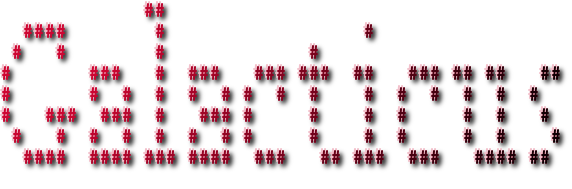
\includegraphics[width=125mm]{GalacticusLogo.png}\\

\Huge Physics Models \normalsize

\docname

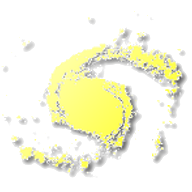
\includegraphics{New_Logo_Galaxy_192_Transparent.png}\\
A semi-analytic galaxy formation code.\\

\copyright\ 2009, 2010 2011, 2012, 2013, 2014, 2015, 2016, 2017, 2018, 2019, 2020, 2021, 2022 Andrew Benson
\end{center}

\tableofcontents

\mainmatter
\pagestyle{headings}

\chapter{Definitions and Conventions Used in \glc}

\glc\ adopts various definitions and conventions internally. These are explained below.

\section{Halo Masses and Dark Matter Mass}

Halo masses require some care in specifying exactly what mass they represent due to the way in which merger trees are typically created. For example, when merger trees are extracted from N-body simulations, those simulations frequently represent \emph{all} matter as collisionless. That is, the simulation contains a density $\Omega_\mathrm{M}=\Omega_\mathrm{DM}+\Omega_\mathrm{b}$ which is the sum of dark and baryonic matter densities, but all of this mass is represented as collisionless particles. Similarly, masses in merger trees built through Monte Carlo techniques typically represent all mass as collisionless.

The exact way in which masses within \glc\ are defined and used in specified in the following subsections.

\subsection{Masses in the Basic Component}

The {\normalfont \ttfamily basic} component (see \S\ref{sec:ComponentBasicProperties}) tracks the mass of each halo as defined in the merger tree. As such, it should be considered to be the mass which the halo would have if baryonic matter behaved just as dark matter. Note that these masses are inclusive of subhalos---that is, the mass of a host halo includes the mass of all of its subhalos.

\subsection{Dark Matter Profiles}

The dark matter profile functions (see \S\ref{phys:darkMatterProfile}) return masses and densities etc. which are normalized to match the mass of the {\normalfont \ttfamily basic} component at the virial radius of the halo. As such, their returned values should be considered to represent the case where baryonic matter behaves as dark matter. This is a convention, and is useful for calculations of large scale structure for example.

\subsection{Galactic Structure Functions}

The various galactic structure functions assume that the masses/densities/etc. reported by the dark matter profile functions should be scaled by a factor $(\Omega_\mathrm{M}-\Omega_\mathrm{b})/\Omega_\mathrm{b}$ to leave only the dark matter part of the profile. Baryonic contributions to the mass/density/etc. will be provided by the components representing those mass distributions.

\subsection{Satellite Virial Orbits}

These functions (see \S\ref{sec:SatelliteVirialOrbits}) typically use the {\normalfont \ttfamily basic} component mass in determining parameters of an orbit, since they are typically calibrated to simulations of collisionless matter only.

\subsection{Satellite Merging Timescales}

These functions (see \S\ref{sec:SatelliteMergingTimescales}) typically use the {\normalfont \ttfamily basic} component mass in determining parameters of an orbit, since they are typically calibrated to simulations of collisionless matter only.

\subsection{Dynamical Friction}

These functions (see \S\ref{sec:satelliteDynamicalFrictionMethod}) evaluate densities through the relevant galactic structure function, and so correctly account for the fraction of the {\normalfont \ttfamily basic} component mass which is in the form of dark matter.

\subsection{Galactic Structure Radius Solvers}

These functions \S\ref{phys:galacticStructureRadiusSolver}) determine the radii of galactic components (such as disk and spheroid), typically by iteratively seeking a solution in which their angular momenta and radii are consistent (assuming rotational support) with the net gravitational potential of the entire system (galaxy plus dark matter halo).

\section{Luminosity Units}

Galaxy luminosities are output in the \gls{ABmagnitude} system, such that a luminosity of $1$ corresponds to an object of $0^\mathrm{th}$ absolute magnitude in the \gls{ABmagnitude} system. This implies that the luminosities are in units of $4.4659\times 10^{13}$~W/Hz.

\section{Peculiar Velocities}\label{sec:GalacticusVelocityDefinitions}

Velocities in \glc\ are always \emph{physical} velocities. When reading merger tree properties (including velocities) from file it is often convenient to store velocities without the Hubble flow contribution, as ``peculiar velocities'', in the file---see \S\ref{sec:ForestHalosGroup} for how to specify whether or not  the velocities included in the file include the Hubble flow or not.

If peculiar velocities are stored it is important to use the same definition of pecular velocity as is used by \glc. Defining $t$ to be physical time and $\mathbf{x}$ to be comoving position, \glc\ uses the conventional definition of peculiar velocity in a cosmological context, namely that it is the deviation of the physical velocity from the Hubble flow. Physical coordinates are given by $\mathbf{r} = a\mathbf{x}$, so the peculiar velocity is
\begin{equation}
\mathbf{v}_\mathrm{pec} \equiv {\mathrm{d} \mathbf{r} \over \mathrm{d} t} - H \mathbf{r} = a {\mathrm{d} \mathbf{x}\over\mathrm{d} t} = {\mathrm{d}\mathbf{x}\over\mathrm{d}\eta},
\end{equation}
where $\mathrm{d}\eta = \mathrm{d}t/a$ is conformal time. 

\section{Gravitational Potentials}\index{potential!gravitational}\index{gravitational potential}

Gravitational potentials are measured in velocity units (i.e. km$^2$/s$^2$), and the arbitrary constant offset is chosen such that the total gravitational potential in any halo at the virial radius is $\Phi(r_\mathrm{virial})=-V_\mathrm{virial}^2$. This choice is made for two reasons:
\begin{enumerate}
\item some mass distributions used have potentials which diverge as $r\rightarrow\infty$, so the usual choice of $\Phi(r) \rightarrow 0$ as $r \rightarrow \infty$ is not applicable;
\item this choice is consistent with the potential at the virial radius of the halo considered as a point mass as is used in Keplerian orbit calculations.
\end{enumerate}
Note that the choice of constant offset for the potential of any mass distribution or galactic component is irrelevant---the galactic structure function which computes potential will ensure that the potential is always offset to match the definition given above.


\chapter{Node Components}

\section{(Supermassive) Black Hole}

\subsection{``Null'' Implementation}

The null black hole implementation defines the same properties as all other black hole implementations, but sets the methods to point to dummy routines (for rate adjustment and derivative computation) or to {\tt null()} for get/set methods. It can be used to effectively switch off black holes. Of course, this is safe only if none of the other active components expect to get or set black hole properties (or if they rely on a sensible implementation of black hole evolution).

\subsection{``Standard'' Implementation}

\subsubsection{Properties}

The standard black hole implementation defines the following properties:
\begin{description}
 \item [{\tt Black\_Hole\_Mass}] The mass of the black hole: $M_\bullet$ {\tt [blackHoleMass]}.
 \item [{\tt Black\_Hole\_Spin}] The spin of the black hole, $j_\bullet$ {\tt [blackHoleSpin]}.
\end{description}

\subsubsection{Initialization}

Black holes are not initialized, they are created (with a seed mass given by {\tt blackHoleSeedMass} and zero spin) as needed.

\subsubsection{Differential Evolution}

In the standard black implementation the mass and spin evolve as:
\begin{eqnarray}
\dot{M}_\bullet &=& (1-\epsilon_{\rm radiation}) \dot{M}_0 \\
\dot{j}_\bullet &=& \dot{j}(M_\bullet,j_\bullet,\dot{M}_0),
\end{eqnarray}
where $\dot{M}_0$ is the rest mass accretion rate, $\epsilon_{\rm radiation}$ is the radiative efficiency of the accretion flow feeding the black hole and $\dot{j}(M_\bullet,j_\bullet,\dot{M}_0)$ is the spin-up function of that accretion flow (see \S\ref{sec:AccretionDisks}). The rest mass accretion rate is computed assuming Bondi-Hoyle-Lyttleton accretion from the spheroid gas reservoir (with an assumed temperature of {\tt [bondiHoyleAccretionTemperatureSpheroid]}) enhanced by a factor of {\tt [bondiHoyleAccretionEnhancementSpheroid]} and from the host halo (with whatever temperature that hot halo temperature profile specifies; see \S\ref{sec:HotHaloTemperature}) enhanced by a factor of {\tt [bondiHoyleAccretionEnhancementHotHalo]}. The rest mass accretion rate is removed (as a mass sink) from the spheroid component. The black hole is assumed to cause feedback in two ways:
\begin{description}
 \item [Radio-mode] Any jet power from the black hole-accretion disk system (see \S\ref{sec:CircumnuclearDisks}) is included in the hot halo heating rate providing that the halo is in the slow cooling regime (i.e. if the cooling radius is smaller than the virial radius; see, for example, \citealt{benson_cold_2010});
 \item [Quasar-mode] A mechanical wind luminosity of \citep{ostriker_momentum_2010}
\begin{equation}
 L_{\rm wind} = \epsilon_{\bullet, wind} \dot{M}_0 \clight^2,
\end{equation}
where $\epsilon_{\bullet wind}=${\tt [blackHoleWindEfficiency]} is the black hole wind efficiency, is added to the gas component of the spheroid (which, presumably, will respond with an outflow for example) if and only if the wind pressure (at the spheroid characteristic radius) is less than the typical thermal pressure in the spheroid gas \citep{ciotti_feedbackcentral_2009}, i.e.
\begin{eqnarray}
 P_{\rm wind} &<& P_{\rm ISM} \nonumber \\
 \frac{1}{2}\rho_{\rm wind} V_{\rm wind}^2 &<& {3 {\rm k_B} T_{\rm ISM} \langle \rho_{\rm ISM}\rangle \over 2 m_{\rm H}}.
\end{eqnarray}
Since $\Omega r^2 \rho_{\rm wind} V_{\rm wind}^3 = L_{\rm wind}$ where $\Omega$ is the solid angle of the wind flow, this can be rearranged to give $\langle\rho_{\rm ISM}\rangle > \rho_{\rm wind, critical}$ where
\begin{equation}
\rho_{\rm wind,critical} = {2 m_{\rm H} L_{\rm wind} \over 3 \Omega r^2 V_{\rm wind} {\rm k_B} T_{\rm ISM}}.
\end{equation}
This critical wind density is computed at the characteristic radius of the spheroid, $r_{\rm spheroid}$, assuming $V_{\rm wind}=10^4$km/s, $T_{\rm ISM}=10^4$K and $\Omega=\pi$, and the \ISM\ density is approximated by
\begin{equation}
 \langle\rho_{\rm ISM}\rangle = {3 M_{\rm gas, spheroid} \over 4 \pi} r_{\rm spheroid}^3.
\end{equation}
For numerical ease, the fraction, $f_{\rm wind}$, of the wind luminosity added to the spheroid is adjusted smoothly through the $\rho_{\rm ISM}\approx\rho_{\rm wind,critical}$ region according to
\begin{equation}
 f_{\rm wind} = \left\{ \begin{array}{ll} 0 & \hbox{ if } x < 0, \\ 3x^2-2x^3 & \hbox{ if } 0 \le x \le 1, \\ 1 & \hbox{ if } x > 1, \end{array} \right.
\end{equation}
where $x=\rho_{\rm ISM}/\rho_{\rm wind,critical}-1/2$.
\end{description}

\subsubsection{Event Evolution}

\noindent\emph{Node mergers:} None.\\

\noindent\emph{Satellite merging:} The black holes in the two merging galaxies are instantaneously merged. Properties are computed using the selected black hole binary merger method (see \S\ref{sec:BlackHoleBinaryMergers}).\\

\noindent\emph{Node promotion:} None.\\

\section{Hot Halo}

\subsection{``Null'' Implementation}

The null hot halo implementation leaves all methods to point to dummy routines (for rate adjustment and derivative computation) or to {\tt null()} for get/set methods. It can be used to effectively switch off hot halos. Of course, this is safe only if none of the other active components expect to get or set hot halo properties (or if they rely on a sensible implementation of hot halo evolution).

\subsection{``Standard'' Implementation}

\subsubsection{Properties}

The standard hot halo implementation defines the following properties:
\begin{description}
 \item [{\tt Hot\_Halo\_Unaccreted\_Mass}] The mass of gas in the hot halo: $M_{\rm failed}$.
 \item [{\tt Hot\_Halo\_Mass}] The mass of gas in the hot halo: $M_{\rm hot}$ {\tt [hotHaloMass]}.
 \item [{\tt Hot\_Halo\_Angular\_Momentum}] The angular momentum of the gas in the hot halo, $J_{\rm hot}$ {\tt [hotHaloAngularMomentum]}.
 \item [{\tt Hot\_Halo\_Abundances}] The mass(es) of heavy elements in gas in the hot halo, $M_{Z, {\rm hot}}$ {\tt [hotHalo\{abundanceName\}]}.
 \item [{\tt Hot\_Halo\_Outflowed\_Mass}] The mass of gas from outflows in the hot halo: $M_{\rm outflowed}$ {\tt [outflowedMass]}.
 \item [{\tt Hot\_Halo\_Outflowed\_Ang\_Mom}] The angular momentum of the outflowed gas in the hot halo, $J_{\rm outflowed}$ {\tt [outflowedAngularMomentum]}.
 \item [{\tt Hot\_Halo\_Outflowed\_Abundances}] The mass(es) of heavy elements in outflowed gas, $M_{Z, {\rm outflowed}}$ {\tt [outflowed\{abundanceName\}]}.
\end{description}
and the following pipes:
\begin{description}
 \item [Energy Input] Energy sent through this pipe is added to the hot halo and used to offset the cooling rate (see below; heat pushed should be in units if $M_\odot$ (km/s)$^2$ Gyr$^{-1}$).
 \item [Cooling Gas] The net cooling rate of gas mass (and metal content and angular momentum) is sent through this pipe. Any component may claim this pipe and connect to it, allowing it to receive the cooling gas.
 \item [Gas Outflow] Galactic components that wish to expel gas due to an outflow can send that mass (plus metals and angular momentum) through this pipe, where it will be received into the hot halo component. 
 \item [Gas Mass Sink] Removes gas (and proportionate amounts of angular momentum and elements) from the hot gas halo.
\end{description}

\subsubsection{Initialization}

At initialization, any nodes with no children are assigned a hot halo mass, and failed accreted mass as dictated by the baryonic accretion method (see \S\ref{sec:AccretionBaryonic}) and angular momentum based on the accreted mass and the halo spin parameter.

\subsubsection{Differential Evolution}

In the standard hot halo implementation the hot gas mass and heavy element mass(es) evolves as:
\begin{eqnarray}
 \dot{M}_{\rm failed} &=& \dot{M}_{\rm failed~accretion} \\
 \dot{M}_{\rm hot} &=& \dot{M}_{\rm accretion} - \dot{M}_{\rm cooling} + \dot{M}_{\rm outflow,return}, \\
 \dot{M}_{Z, {\rm hot}} &=& - \dot{M}_{\rm cooling} {M_{Z, {\rm hot}}\over M_{\rm hot}} + \dot{M}_{Z, {\rm outflow,return}}, \\
\end{eqnarray}
where $\dot{M}_{\rm accretion}$ is the rate of growth of the hot component due to accretion from the \IGM\ and $\dot{M}_{\rm failed~accretion}$ is the rate of failed accretion from the \IGM\ (these may include a component due to transfer of mass from the failed to accreted reservoirs) and $\dot{M}_{\rm cooling}$ is the rate of mass loss from the hot halo due to cooling (see \S\ref{sec:CoolingRate}) minus any heating rate defined as
\begin{equation}
 \dot{M}_{\rm heating} = \dot{E}{\rm input} / V_{\rm virial}^2,
\end{equation}
where $\dot{E}$ is the rate at which energy is being sent through the ``energy input'' pipe and $V_{\rm virial}$ is the virial velocity of the halo.\footnote{The net cooling rate is never allowed to drop below zero. If the mass heating rate exceeds the mass cooling rate then the excess energy is not used.} The angular momentum of the hot gas evolves as:
\begin{equation}
 \dot{J}_{\rm hot} = \dot{M}_{\rm accretion} {\dot{J}_{\rm node} \over \dot{M}_{\rm node}} - \dot{M}_{\rm cooling} r_{\rm cool} V_{\rm rotate} + \dot{J}_{\rm outflow,return},
\end{equation}
where $\dot{M}_{\rm node}$ and $\dot{J}_{\rm node}$ are defined in \S\ref{sec:ComponentBasicProperties}. For the outflowed components:
\begin{eqnarray}
 \dot{M}_{\rm outflowed} &=& - \dot{M}_{\rm outflow,return} + \dot{M}_{\rm outflows}, \\
 \dot{M}_{Z, {\rm outflowed}} &=& - \dot{M}_{Z, {\rm outflow,return}} + \dot{M}_{Z, {\rm outflows}}, \\
\end{eqnarray}
and:
\begin{equation}
 \dot{J}_{\rm outflowed} = - \dot{J}_{\rm outflow,return} + \dot{J}_{\rm outflows}.
\end{equation}
In the above
\begin{equation}
 \dot{M}|\dot{M}_Z|\dot{J}_{\rm outflow,return} = \alpha_{\rm outflow~return~rate} {M|M_Z|J_{\rm outflowed}\over \tau_{\rm dynamical, halo}},
\end{equation}
where $\alpha_{\rm outflow~return~rate}=(${\tt hotHaloOutflowReturnRate}) is an input parameter controlling the rate at which gas flows from the outflowed to hot reservoirs, and $\dot{M}|\dot{M}_Z|\dot{J}_{\rm outflows}$ are the net rates of outflow from any components in the node.

\subsubsection{Event Evolution}

\noindent\emph{Node mergers:} If the {\tt starveSatellites} parameter is true, then any hot halo properties of the minor node are added to those of the major node and the hot halo component removed from the minor node. Additionally in this case, any material outflowed from the the satellite galaxy to its hot halo is transferred to the hot halo of the host dark matter halo after each timestep.\\

\noindent\emph{Satellite merging:} If the {\tt starveSatellites} parameter is false, then any hot halo properties of the satellite node are added to those of the host node and the hot halo component removed from the satellite node.\\

\noindent\emph{Node promotion:} Any hot halo properties of the parent node are added to those of the node prior to promotion.\\

\section{Galactic Disk}

\subsection{``Null'' Implementation}

The null disk implementation leaves all methods to point to dummy routines (for rate adjustment and derivative computation) or to {\tt null()} for get/set methods. It can be used to effectively switch off disks. Of course, this is safe only if none of the other active components expect to get or set disk properties (or if they rely on a sensible implementation of disk evolution).

\subsection{``Exponential'' Implementation}\label{sec:DiskExponential}

This implementation assumes a disk with an exponential surface density profile in which stars trace gas.

\subsubsection{Properties}

The exponential galactic disk implementation defines the following properties:
\begin{description}
 \item [{\tt Disk\_Gas\_Mass}] The mass of gas in the disk: $M_{\rm disk, gas}$ [{\tt diskGasMass}].
 \item [{\tt Disk\_Gas\_Abundances}] The mass of elements in the gaseous disk: $M_{Z, {\rm disk, gas}}$ [{\tt diskGas\{abundanceName\}}].
 \item [{\tt Disk\_Stellar\_Mass}] The mass of stars in the disk: $M_{\rm disk, stars}$ [{\tt diskStellarMass}].
 \item [{\tt Disk\_Stellar\_Abundances}] The mass of elements in the stellar disk: $M_{Z, {\rm disk, stars}}$ [{\tt diskStellar\{abundanceName\}}].
 \item [{\tt Disk\_Stellar\_Luminosities}] The luminosities (in multiple bands) of the stellar disk: $L_{\rm disk, stars}$ [{\tt diskStellar\{luminosityName\}}].
 \item [{\tt Disk\_Angular\_Momentum}] The angular momentum of the disk, $J_{\rm disk}$ [{\tt diskAngularMomentum}].
 \item [{\tt Disk\_Radius}] The radial scale length of the disk, $R_{\rm disk}$ [{\tt diskScaleLength}].
 \item [{\tt Disk\_Velocity}] The circular velocity of the disk at $R_{\rm disk}$, $V_{\rm disk}$ [{\tt diskCircularVelocity}].
\end{description}

\subsubsection{Initialization}

No initialization is performed---disks are created as needed.

\subsubsection{Differential Evolution}

In the exponential galactic disk implementation the gas mass evolves as:
\begin{equation}
 \dot{M}_{\rm disk, gas} = \dot{M}_{\rm cooling} - \dot{M}_{\rm outflow, disk} - \dot{M}_{\rm stars, disk} - M_{\rm disk, gas}/\tau_{\rm bar},
\end{equation}
where the rate of change of stellar mass is
\begin{equation}
 \dot{M}_{\rm stars, disk} = \Psi - \dot{R} - M_{\rm stars,disk}/\tau_{\rm bar},
\end{equation}
with
\begin{equation}
 \Psi = {M_{\rm disk, gas} \over \tau_{\rm disk, star~formation}}
\end{equation}
with $\tau_{\rm disk, star~formation}$ being the star formation timescale and $\dot{R}$ is the rate of mass recycling from stars and $\tau_{\rm bar}$ is a bar instability timescale (see \S\ref{sec:DiskStability}). The mass removed from the disk by the bar instability mechanism is added to the active spheroid component.
Element abundances (including total metals) evolve according to:
\begin{equation}
  \dot{M}_{Z, {\rm disk, gas}} = \dot{M}_{Z {\rm cooling}} - \dot{M}_{Z, {\rm outflow, disk}} - \dot{M}_{Z, {\rm stars, disk}} + \dot{y},
\end{equation}
and
\begin{equation}
 \dot{M}_{Z, {\rm stars, disk}} = \Psi {M_{Z, {\rm disk, gas}} \over M_{\rm disk, gas}} - \dot{R}_Z
\end{equation}
where $\dot{y}$ is the rate of element yield from stars and $\dot{R}_Z$ is the rate of element recycling. The angular momentum evolves as:
\begin{equation}
 \dot{J}_{\rm disk} = \dot{J}_{\rm cooling} - \left[ \dot{M}_{\rm outflow, disk} + {M_{\rm disk, gas}  + M_{\rm disk, stars} \over \tau_{\rm bar}}\right] {J_{\rm disk} \over M_{\rm disk, gas} + M_{\rm disk, stars}}.
\end{equation}
The outflow rate, $\dot{M}_{\rm outflow, disk}$, is computed for the current star formation rate and gas properties by the stellar properties subsystem (see \S\ref{sec:StellarPopulationProperties}), but is not allowed to exceed $M_{\rm gas, disk}/ \alpha_{\rm outflow minimum, disk} \tau_{\rm disk, dynamical}$, where $\tau_{\rm disk, dynamical}=R_{\rm disk}/V_{\rm disk}$ is the dynamical time of the disk and $\alpha_{\rm outflow minimum, disk}=${\tt [diskOutflowTimescaleMinimum]} is the shortest timescale (in units of the dynamical timescale) on which gas can be removed from the disk. This limit prevents the disk being depleted on arbitrarily short timescales.

\subsubsection{Event Evolution}

\noindent\emph{Node mergers:} None\\

\noindent\emph{Satellite merging:} Disks may be destroyed (or, potentially, created or otherwise modified) as the result of a satellite merging event, as dictated by the selected merger remnant mass movement method (see \S\ref{sec:MergingMassMovements}).\\

\noindent\emph{Node promotion:} None\\

\section{Galactic Spheroid}

\subsection{``Null'' Implementation}

The null spheroid implementation leaves all methods to point to dummy routines (for rate adjustment and derivative computation) or to {\tt null()} for get/set methods. It can be used to effectively switch off spheroids. Of course, this is safe only if none of the other active components expect to get or set spheroid properties (or if they rely on a sensible implementation of spheroid evolution).

\subsection{``Hernquist'' Implementation}

This implementation assumes a Hernquist profile \citep{hernquist_analytical_1990} for the spheroidal component of a galaxy in which stars trace gas.

\subsubsection{Properties}

The Hernquist galactic spheroid implementation defines the following properties:
\begin{description}
 \item [{\tt Spheroid\_Gas\_Mass}] The mass of gas in the spheroid: $M_{\rm spheroid, gas}$ [{\tt spheroidGasMass}].
 \item [{\tt Spheroid\_Gas\_Abundances}] The mass of elements in the gaseous spheroid: $M_{Z, {\rm spheroid, gas}}$ [{\tt spheroidGas\{abundanceName\}}].
 \item [{\tt Spheroid\_Stellar\_Mass}] The mass of stars in the spheroid: $M_{\rm spheroid, stars}$ [{\tt spheroidStellarMass}].
 \item [{\tt Spheroid\_Stellar\_Abundances}] The mass of elements in the stellar spheroid: $M_{Z, {\rm spheroid, stars}}$ [{\tt spheroidStellar\{abundanceName\}}].
 \item [{\tt Spheroid\_Stellar\_Luminosities}] The luminosities (in multiple bands) of the stellar spheroid: $L_{\rm spheroid, stars}$ [{\tt spheroidStellar\{luminosityName\}}].
 \item [{\tt Spheroid\_Angular\_Momentum}] The pseudo-angular momentum\footnote{Effectively the angular momentum that the spheroid would have, were it rotationally supported rather than pressure supported.} of the spheroid, $J_{\rm spheroid}$ [{\tt spheroidAngularMomentum}].
 \item [{\tt Spheroid\_Radius}] The radial scale length of the spheroid, $r_{\rm spheroid}$ [{\tt spheroidScaleLength}].
 \item [{\tt Spheroid\_Velocity}] The circular velocity of the spheroid at $r_{\rm spheroid}$, $V_{\rm spheroid}$ [{\tt spheroidCircularVelocity}].
\end{description}
and the following pipes:
\begin{description}
 \item [{\tt Tree\_Node\_Spheroid\_Gas\_Energy\_Input}] Energy sent through this pipe is added to the gas of the spheroid and will result in an outflow (see below). Input energy should be in units of $M_\odot$ km$^2$ s$^{-2}$ Gyr$^{-1}$ and must be positive (energy cannot be removed from the gas via this pipe).
 \item [{\tt Tree\_Node\_Spheroid\_Gas\_Sink}] Removes gas (and proportionate amounts of angular momentum and elements) from the spheroid gas. Removed mass should be in units of $M_\odot$ and must be positive (a negative mass sink would add mass to the spheroid which is not allowed via this pipe).
\end{description}

\subsubsection{Initialization}

No initialization is performed---spheroids are created as needed.

\subsubsection{Differential Evolution}

In the Hernquist galactic spheroid implementation the gas mass evolves as\footnote{There may be an additional contribution to the mass and angular momentum rates of change in the spheroid due to material transferred from the disk component via the bar instability mechanism (see \S\protect\ref{sec:DiskExponential}). This is not included here as it is not intrinsic to this specific spheroid implementation---it is handled explicitly by the disk component and so applies equally to any spheroid component implementation.}:
\begin{equation}
 \dot{M}_{\rm spheroid, gas} = - \dot{M}_{\rm outflow, spheroid} - \dot{M}_{\rm stars, spheroid},
\end{equation}
where the rate of change of stellar mass is
\begin{equation}
 \dot{M}_{\rm stars, spheroid} = \Psi - \dot{R}
\end{equation}
with
\begin{equation}
 \Psi = {M_{\rm spheroid, gas} \over \tau_{\rm spheroid, star~formation}}
\end{equation}
with $\tau_{\rm spheroid, star~formation}$ being the star formation timescale and $\dot{R}$ is the rate of mass recycling from stars.
Element abundances (including total metals) evolve according to:
\begin{equation}
  \dot{M}_{Z, {\rm spheroid, gas}} = - \dot{M}_{Z, {\rm outflow, spheroid}} - \dot{M}_{Z, {\rm stars, spheroid}} + \dot{y},
\end{equation}
and
\begin{equation}
 \dot{M}_{Z, {\rm stars, spheroid}} = \Psi {M_{Z, {\rm spheroid, gas}} \over M_{\rm spheroid, gas}} - \dot{R}_Z
\end{equation}
where $\dot{y}$ is the rate of element yield from stars and $\dot{R}_Z$ is the rate of element recycling. The angular momentum evolves as:
\begin{equation}
 \dot{J}_{\rm spheroid} = \dot{M}_{\rm outflow, spheroid} {J_{\rm spheroid} \over M_{\rm spheroid, gas} + M_{\rm spheroid, stars}}.
\end{equation}
The outflow rate, $\dot{M}_{\rm outflow, spheroid}$, is computed for the current star formation rate and gas properties by the stellar properties subsystem (see \S\ref{sec:StellarPopulationProperties}), and which is not allowed to exceed $M_{\rm gas, spheroid}/ \alpha_{\rm outflow minimum, spheroid} \tau_{\rm spheroid, dynamical}$, where $\tau_{\rm spheroid, dynamical}=r_{\rm spheroid}/V_{\rm spheroid}$ is the dynamical time of the spheroid and $\alpha_{\rm outflow minimum, spheroid}=${\tt [spheroidOutflowTimescaleMinimum]} is the shortest timescale (in units of the dynamical timescale) on which gas can be removed from the spheroid (this limit prevents the spheroid being depleted on arbitrarily short timescales), with an additional contribution given by
\begin{equation}
 \dot{M}_{\rm outflow, spheroid} = \beta_{\rm spheroid, energy} {\dot{E}_{\rm gas, spheroid} \over V_{\rm spheroid}^2}
\end{equation}
where $\beta_{\rm spheroid, energy}=${\tt [spheroidEnergeticOutflowMassRate]} is an input parameter, and $\dot{E}_{\rm gas,spheroid}$ is any input energy sent through the {\tt Tree\_Node\_Spheroid\_Gas\_Energy\_Input} pipe.

\subsubsection{Event Evolution}

\noindent\emph{Node mergers:} None\\

\noindent\emph{Satellite merging:} Spheroids may be created as the result of a satellite merging event, as dictated by the selected merger remnant mass movement method (see \S\ref{sec:satelliteMergerMassMovementMethod}).\\

\noindent\emph{Node promotion:} None.\\

\section{Basic Properties}\label{sec:ComponentBasicProperties}

Basic properties are the total mass of a node and the cosmic time at which it currently exists.

\subsection{``Simple'' Implemenation}

\subsubsection{Properties}

The simple basic properties implementation defines the following properties:
\begin{description}
 \item [{\tt Mass}] The total mass of the node: $M_{\rm node}$ [{\tt nodeMass}].
 \item [{\tt Time}] The time at which the node is defined: $t_{\rm node}$.
 \item [{\tt TimeLastIsolated}] The time at which the node was last an isolated halo (i.e. not a subhalo): [\tt nodeTimeLastIsolated].
\end{description}

\subsubsection{Initialization}

All basic properties are required to be initialized by the merger tree construction routine.

\subsubsection{Differential Evolution}

Properties are evolved according to:
\begin{eqnarray}
 \dot{M}_{\rm node} &=& \left\{\begin{array}{ll}{M_{\rm node, parent} - M_{\rm node} \over t_{\rm node, parent} - t_{\rm node}} & \hbox{ if primary progenitor} \\ 0 & \hbox{ otherwise}, \end{array} \right. \\
 \dot{t}_{\rm node} &=& 1,
\end{eqnarray}
where the ``parent'' subscript indicates a property of the parent node in the merger tree.

\subsubsection{Event Evolution}

\noindent\emph{Node mergers:} None.\\

\noindent\emph{Satellite merging:} None.\\

\noindent\emph{Node promotion:} $M_{\rm node}$ is updated to the node mass of the parent prior to promotion.\\

\section{Position}\label{sec:ComponentPosition}

The position component implements the position and velocity of each galaxy.

\subsection{``Null'' Implementation}

The null position implementation leaves all methods to point to dummy routines (for rate adjustment and derivative computation) or to {\tt null()} for get/set methods. It can be used to effectively switch off positions. Of course, this is safe only if none of the other active components, functions or tasks expect to get or set position properties (or if they rely on a sensible implementation of position evolution).

\subsection{``Preset'' Implemenation}

\subsubsection{Properties}

The preset position implementation defines the following properties:
\begin{description}
 \item [{\tt Position}] The 3-D position of the node: ${\bf x}$ [{\tt position[X|Y|Z]}].
 \item [{\tt Velocity}] The 3-D velocity of the node: ${\bf v}$ [{\tt velocity[X|Y|Z]}].
 \item [{\tt Position\_6D\_History}] The history of the node's position in 6-D phase space, usually used for satellite nodes.
\end{description}

\subsubsection{Initialization}

None---all properties are assumed to have been preset, usually by the merger tree construction routine.

\subsubsection{Differential Evolution}

None. Positions and velocities do not evolve for a given node. When output, if a 6-D position history is available than the position and velocity from the history entry closest to the output time will be used\footnote{While interpolation could be used this is usually a bad idea. For nodes that are satellites in a halo for example, no simple interpolation algorithm can correctly account for the complex orbital dynamics by which the position and velocity is actually evolving.}.

\subsubsection{Event Evolution}

\noindent\emph{Node mergers:} None.\\

\noindent\emph{Satellite merging:} None.\\

\noindent\emph{Node promotion:} The position and velocity are updated to those of the parent node.\\

\section{Satellite Node Orbit}

This component tracks the orbital properties of subhalos.

\subsection{``Preset'' Implementation}

\subsubsection{Properties}

The preset satellite orbit implementation defines the following properties:
\begin{description}
 \item [{\tt Satellite\_Merge\_Time}] The time until the satellite will merge with its host: $t_{\rm satellite, merge}$ [{\tt timeToMerge}].
 \item [{\tt Satellite\_Time\_Of\_Merging}] The cosmological time at which the satellite will merge with its host: $T_{\rm satellite, merge}$.
 \item [{\tt Bound\_Mass}] The remaining, total bound mass of the satellite (this property is read only---it is determined from the {\tt Bound\_Mass\_History} property).
 \item [{\tt Bound\_Mass\_History}] A history time-series of the total bound mass of the satellite.
\end{description}

Note that the {\tt Satellite\_Merge\_Time} and {\tt Satellite\_Time\_Of\_Merging} effectively provide the same information. For that reason, setting one of them will automatically set the other accordingly.

\subsubsection{Initialization}

None. This method assumes that merging times and bound mass histories will be set externally (usually when the merger tree is constructed).

\subsubsection{Differential Evolution}

None.

\subsubsection{Event Evolution}

\noindent\emph{Node mergers:} None.\\

\noindent\emph{Satellite merging:} None.\\

\noindent\emph{Node promotion:} None.\\

\subsection{``Simple'' Implementation}

\subsubsection{Properties}

The simple satellite orbit implementation defines the following properties:
\begin{description}
 \item [{\tt Satellite\_Merge\_Time}] The time until the satellite will merge with its host: $t_{\rm satellite, merge}$ [{\tt timeToMerge}].
\end{description}

\subsubsection{Initialization}

None.

\subsubsection{Differential Evolution}

Properties are evolved according to:
\begin{equation}
 \dot{t}_{\rm satellite, merge} = -1.
\end{equation}

\subsubsection{Event Evolution}

\noindent\emph{Node mergers:} The component is created and the time to merging is assigned a value.\\

\noindent\emph{Satellite merging:} None.\\

\noindent\emph{Node promotion:} Not applicable (component only exists for satellite nodes).\\

\section{Dark Matter Halo Spin}

\subsection{``Null'' Implementation}

The null spin implementation leaves all methods to point to dummy routines (for rate adjustment and derivative computation) or to {\tt null()} for get/set methods. It can be used to effectively switch off spins. Of course, this is safe only if none of the other active components expect to get or set spin properties (or if they rely on a sensible implementation of spin evolution).

\subsection{``Random'' Implementation}

\subsubsection{Properties}

The random dark matter halo spin implementation defines the following properties:
\begin{description}
 \item [{\tt Spin}] The spin parameter of the halo: $\lambda$ [{\tt nodeSpin}].
\end{description}

\subsubsection{Initialization}

The spin parameter of each node, if not already assigned, is selected at random from a distribution of spin parameters. This value is assigned to the earliest progenitor of the halo traced along its primary branch. The value is then propagated forward along the primary branch until the node mass exceeds that of the node for which the spin was selected by a factor of {\tt [randomSpinResetMassFactor]}, at which point a new spin is selected at random, and the process repeated until the end of the branch is reached. 

\subsubsection{Differential Evolution}

The spin parameter does not evolve.

\subsubsection{Event Evolution}

\noindent\emph{Node mergers:} None.\\

\noindent\emph{Satellite merging:} None.\\

\noindent\emph{Node promotion:} The spin is updated to equal that of the parent node. (The two will differ only if this is a case where the new halo node was sufficiently more massive than the node for which a spin was last selected that a new spin value was chosen.)\\

\section{Dark Matter Profile}

This component stores dynamic properties associated with dark matter halo density profiles.

\subsection{``Null'' Implementation}

The null profile implementation leaves all methods to point to dummy routines (for rate adjustment and derivative computation) or to {\tt null()} for get/set methods. It can be used to effectively switch off profiles. Of course, this is safe only if none of the other active components expect to get or set profile properties (or if they rely on a sensible implementation of profile evolution).

\subsection{``Scale'' Implementation}

\subsubsection{Properties}

The scale dark matter profile implementation defines the following properties:
\begin{description}
 \item [{\tt Scale}] The scale length of the density profile [{\tt darkMatterScaleRadius}];
 \item [{\tt Scale\_Growth\_Rate}] The growth rate of the scale length of the density profile.
\end{description}

\subsubsection{Initialization}

The scale length of each node, if not already assigned, is assigned using the concentration parameter function (see \S\ref{sec:DarkMatterProfileConcentration}), but is not allowed to drop below {\tt [darkMatterProfileMinimumConcentration]}, such that the scale length is equal to the virial radius divided by that concentration. The value is propagated in both directions along the primary child branch from the node.

\subsubsection{Differential Evolution}

The scale radius does not evolve.

\subsubsection{Event Evolution}

\noindent\emph{Node mergers:} None.\\

\noindent\emph{Satellite merging:} None.\\

\noindent\emph{Node promotion:} None.\\



\chapter{Functions}\label{sec:Functions}

\IfFileExists{./autoPhysics.tex}{\input{autoPhysics}}{}



\backmatter

\bibliographystyle{plainnat}
\bibliography{GalacticusAccented}

\printglossaries

\citeindextrue
\printindex

\end{document}
